\documentclass[a4]{scrartcl}

% \usepackage[ngerman]{babel}
\usepackage[utf8]{inputenc}
\usepackage{mathtools}
\usepackage{amsmath}
\usepackage{amssymb}
\usepackage{geometry}
\usepackage{scrlayer-scrpage}
\usepackage{float}
\usepackage{xcolor}
\pagestyle{scrheadings}
\clearscrheadfoot

\usepackage[backend=biber, maxbibnames=99]{biblatex}
\addbibresource{references.bib}

\setlength{\parindent}{0cm}


\geometry{
  paper=a4paper, % Change to letterpaper for US letter
  top=2cm, % Top margin
  bottom=1.5cm, % Bottom margin
  left=2cm, % Left margin
  right=3cm, % Right margin
}

\ohead{\\
Pina Kolling\\
piko0011}

\usepackage[framemethod=TikZ]{mdframed}

% Style %
\mdfdefinestyle{enviStyle}{
   innertopmargin = 10pt,
  linewidth      = 1pt,
  frametitlerule = true,
  roundcorner    = 2pt%
}


\newenvironment{CountingDefinition}[2][]{%
   \ifstrempty{#1}%
   {\mdfsetup{%
      frametitle={{\strut ~}}}
   }%
   {\mdfsetup{%
      frametitle={{\strut ~#1}}}%
   }%
   \mdfsetup{
      nobreak                   = true,
     linecolor                 = gray,
    frametitlebackgroundcolor = gray!50,
    style                     = enviStyle
   }
   \begin{mdframed}[]\relax%
   \label{#2}}{\end{mdframed}}

\begin{document}

\section*{Summary: Lecture 9}

Summary for the chapter \textit{10.3}. \cite{book, CC}


% First part in more detail. Second part (total functions) read and summarize a little.



%------------------------------------------------------------

\subsection*{Function problems}

\begin{CountingDefinition}[Function problem]{def:validLabelPlacement}
Finding a specific solution to a problem if possible, else return \textit{no}.
\end{CountingDefinition}

\begin{itemize}
\item focus so far: languages deciding decision problems
\item give \textit{yes} or \textit{no} as answer
\item now: focus on finding a solution:
\begin{itemize}
\item find satisfying truth assignment for a boolean expression
\item find optimal tour for \textsc{Tsp}
\item[$\rightarrow$] function problems \\
\end{itemize}

\item decision problems are helpful for negative results of function problems
\item complexity of the decision problem helps to specify the complexity of the corresponding function problem
\end{itemize}









%------------------------------------------------------------

\subsection*{SAT and FSAT}

\begin{CountingDefinition}[\textsc{SAT}]{def:validLabelPlacement}
The \textsc{Sat} (satisfiability) problem is the problem of determining if there exists an interpretation that satisfies a given Boolean formula. \cite{GTI}
\end{CountingDefinition}


\begin{CountingDefinition}[\textsc{FSAT}]{def:validLabelPlacement}
The \textsc{FSat} (satisfiability) problem is a function problem. 

\ \\
Given a boolean expression $\phi$.

If $\phi$ is satisfiable, return a satisfying truth assignment and otherwise return \textit{no}.
\end{CountingDefinition}


\begin{itemize}
\item for input $\phi$ there might be no satisying truth assignment $\phi \notin \textsc{Sat}$
\begin{itemize}
\item return \textit{no}
\end{itemize}
\item for input $\phi$ there might be more than one satisying truth assignment 
\begin{itemize}
\item return any satisfying truth assignment
\end{itemize}
\item if \textsc{Sat} can be solved in polynomial time, \textsc{FSat} can be solved in polynomial time, too

\end{itemize}

Algorithm for \textsc{FSat}:

\begin{itemize}
\item expression $\phi$ with variables $x_1, ... , x_n$

\item ask if $\phi$ is satisfiable ($\phi \in \textsc{Sat}$):
\begin{itemize}
\item if \textit{no}: stop and return \textit{no}
\item if \textit{yes}: come up with satisying truth assignment

\begin{itemize}
\item consider two expressions: $\phi[x_1 = \text{true}]$ and $\phi[x_1 = \text{false}]$
\item check which one is satisfiable ($\phi[x_1 = \text{true}] \in \textsc{Sat}$ or $\phi[x_1 = \text{false}] \in \textsc{Sat}$) \\
(if both are, chose one)
\item substitute the value of $x_1$ in $\phi$ 
\item continue with $x_2$
\item at most $2n$ calls to find the satisfying truth assignment
\end{itemize}

\end{itemize}

\end{itemize}

Algorithm for \textsc{FSat} as pseudo code:

\begin{figure}[H]
\begin{center}
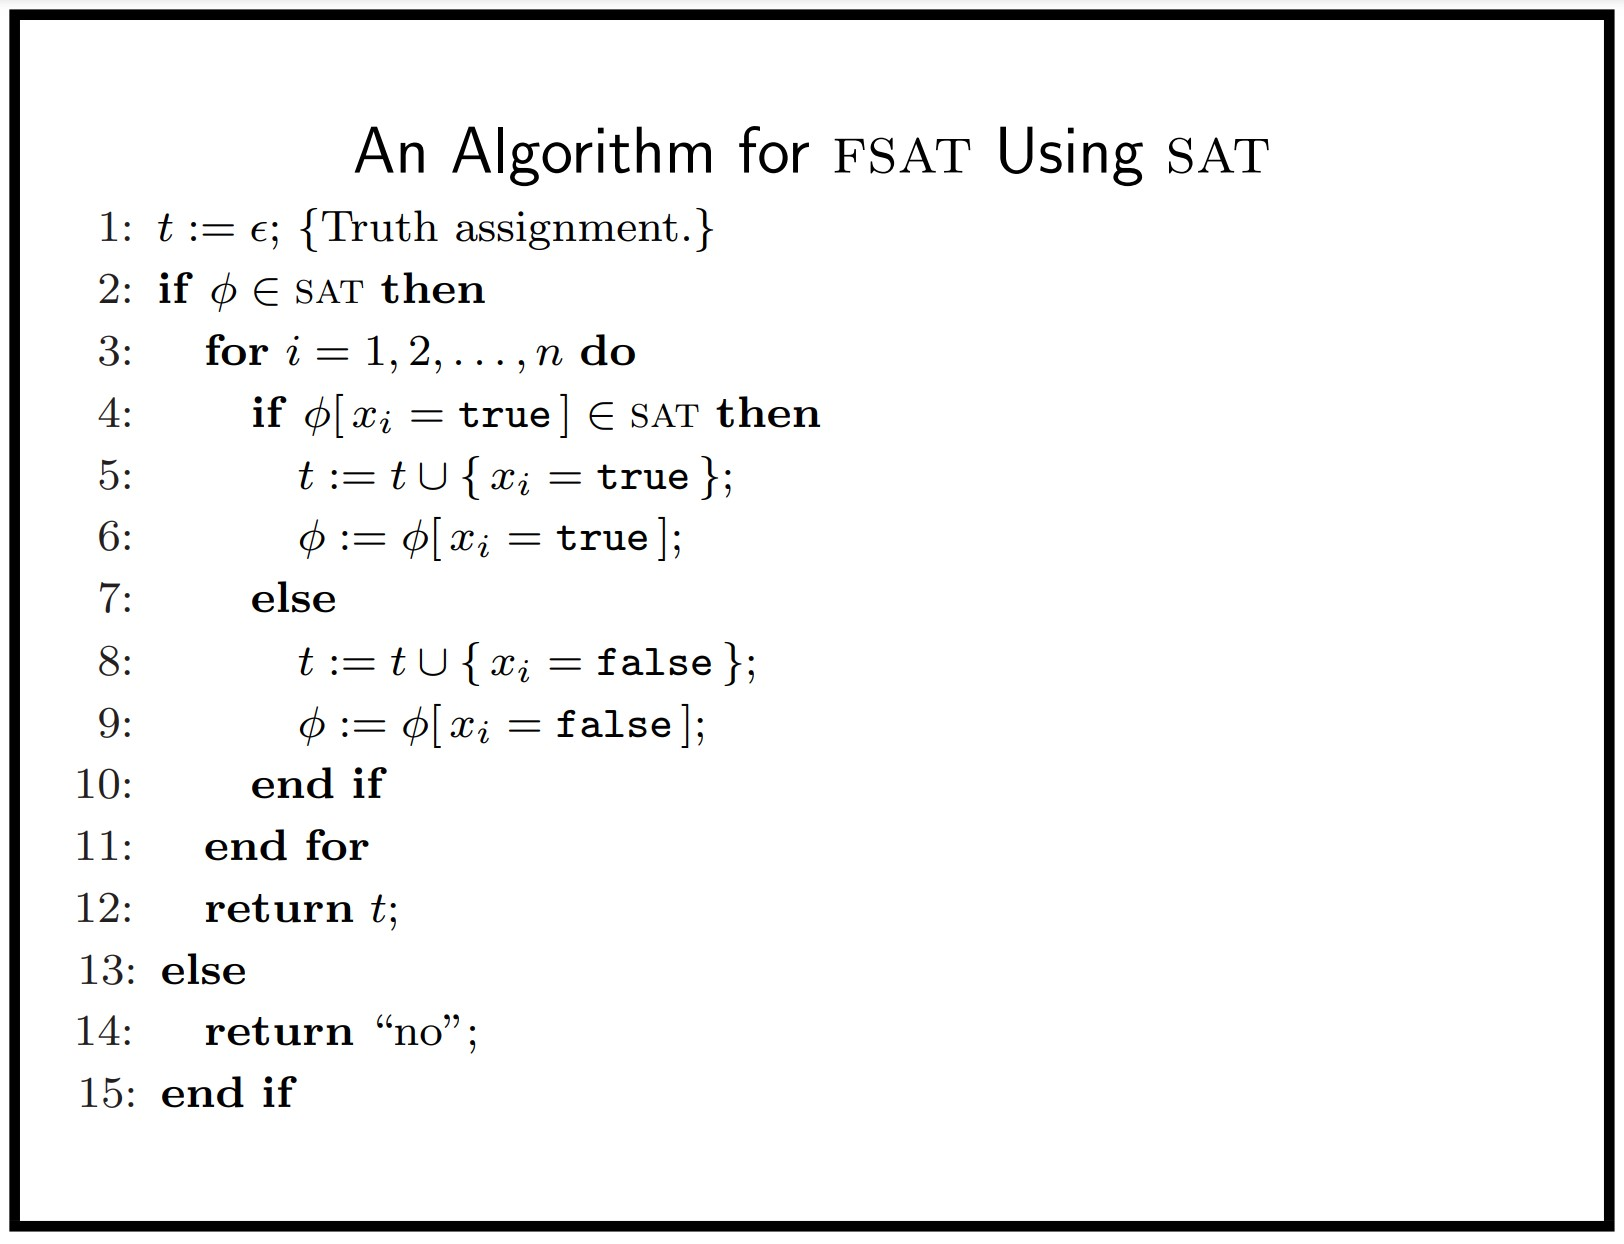
\includegraphics[scale=0.6]{fsat.jpg}
\end{center}
\caption{\textsc{FSat} algorithm as pseudo code \cite{RCV}}
\end{figure}



Self-reducibilty:

\begin{itemize}
\item 
\end{itemize}


\color{red} TODO \\
Self-reducibility \\ \\
\color{black}
\color{violet} Questions: \\

\begin{itemize}
\item Book \cite{book}:

\textsc{FSat} draws its difficulty precisely from the possibility that there may be no truth assignment satisfying the given expression.

\item[$\rightarrow$] Why is the difficulty coming from the possibility that there might be no truth assignment? It would in the first check of $\phi \in \textsc{Sat}$ return \textit{no} and terminate? 
\end{itemize}

\color{black}



%------------------------------------------------------------

\subsection*{TSP and TSP(D)}



\begin{CountingDefinition}[\textsc{TSP(D)}]{def:validLabelPlacement}
Given a list of cities and the distances between each pair of cities.

\ \\ 
Is there a possible route of length $k$ that visits each city exactly once and returns to the origin city?
\end{CountingDefinition}


\begin{CountingDefinition}[\textsc{TSP}]{def:validLabelPlacement}
Given a list of cities and the distances between each pair of cities.

\ \\
What is the shortest possible route that visits each city exactly once and returns to the origin city?
\end{CountingDefinition}

\begin{itemize}
\item solve \textsc{Tsp} with an algorithm for \textsc{Tsp(D)}
\item find optimum cost $C$ of the tour with binary search (between 0 and $2^n$)
\item remove one intercity distance at a time to check if it is part of the optimal tour
\item after $n^2$ calls only entries of the distance matrix are there that are used for the optimum tour
\end{itemize}


\color{red} TODO \\
algorithm TSP (?) \\
maybe example (?) \\
\color{black}
\color{violet} Questions:
\color{black}









%------------------------------------------------------------

\subsection*{FP and FNP}

\begin{CountingDefinition}[Lanugage $L$]{def:validLabelPlacement}
$L= \{ x: (x,y) \in R \textit{ for some } y \}$ \ 
\\
$L$ gets an input $x$ and finds a $y$ with $((x,y) \in R$ and the relation $R \subseteq \Sigma^* \times \Sigma^*$.
\end{CountingDefinition}

\begin{CountingDefinition}[NP]{def:validLabelPlacement}
The language $L \subseteq \Sigma^*$ is in NP only if there is a polynomially decidable and polynomially balanced relation $R$ such that  $L= \{ x: (x,y) \in R \textit{ for some } y \}$.
\end{CountingDefinition}

Relationship between decision and function problems:
\begin{itemize}
\item $L$ is a lanuage in NP
\begin{itemize}
\item \textbf{Decision problem:} \\
There is a string $y$ with $R(x,y)$ only if $x \in L$.
\item \textbf{Function problem:} \\
Given $x$, find a string $y$ such that $R(x,y)$ if it exists, else return \textit{no}.
\end{itemize}

\end{itemize}

\begin{CountingDefinition}[FNP]{def:validLabelPlacement}
Class of all function problems asspciated with languages in NP.
\end{CountingDefinition}


\begin{CountingDefinition}[FP]{def:validLabelPlacement}
FP is the subclass of FNP that contains function problems, that can be solved in polynomial time.
\end{CountingDefinition}

\textbf{Examples:}
\begin{itemize}
\item \textsc{FSat} is in FNP but expected to be in FP
\item \textsc{HornSat} is in FP
\item \textsc{BipartiteGraph} is in FP
\end{itemize}











%------------------------------------------------------------

\subsection*{Reductions between function problems}

\begin{CountingDefinition}[Reductions between function problems]{def:validLabelPlacement}
A function problem $A$ reduces to a function problem $B$ if the following holds:
\begin{itemize}
\item $R$ and $S$ are string functions, $x$ and $z$ are strings
\item If $x$ is an instance of $A$ then $R(x)$ is an instance of $B$.
\item If $z$ is a correct output of $R(x)$, then $S(z)$ is a correct output of $x$.
\end{itemize}

\end{CountingDefinition}

\begin{itemize}
\item $R$ produces an instance $R(x)$ of the function problem $B$
\item $S(z)$ is an constructed output for $x$ from any correct output $z$ of $R(x)$
\item translate answers back to the original problem
\item reduction is a pair $(R,S)$:
\begin{itemize}
\item $R$ translates input $x$ to input $x'$
\item $S$ translates result $z'$ to result $z$
\end{itemize}

\item a function problem $A$ is complete for a class F$C$ if it is in F$C$ and all problems in that class reduce to $A$
\item FP and FNP are closed under reduction
\item reductions of function problems compose
\end{itemize}










%------------------------------------------------------------

\subsection*{How to prove FP = FNP?}



\begin{itemize}
\item FP = FNP only if P = NP

\item Computing a satisfying assignment bit by bit


\item \textsc{Sat$'$} is a formular $\varphi$ plus an assignment that satisfies $\varphi$
\item assignment as clauses that connects the single variables or their negation with $\land$
\end{itemize}

\color{red} TODO \\
\color{black}
\color{violet} Questions:
\color{black}









%------------------------------------------------------------

\subsection*{If FP=FNP optimuzation problems become easy}

\begin{CountingDefinition}[Title]{def:validLabelPlacement}
Content
\end{CountingDefinition}


\begin{itemize}
\item 
\end{itemize}

\color{red} TODO \\
\color{black}
\color{violet} Questions:
\color{black}









%------------------------------------------------------------

\subsection*{Cryptography}

Cryptography argument \cite{DD, book, GTI}: 
\begin{itemize}
\item P vs. NP problem is an unsolved problem
\item currently clear: a correct solution to an NP problem can be checked for correctness in polynomial time
\item experts wish NP problems to remain almost unsolvable because of cryptography
\item complexity in cryptography is not only desirable, but necessary
\item important to know that most encryption methods used today are based solely on the fact that the effort to \textit{guess} the key is too high \\
$\rightarrow$ problem of \textit{guessing} is an NP problem
\item proof of the solvability of NP problems means the end of all currently used encryption methods
\item[$\rightarrow$] cryptographic argument: if P=NP, no safe encoding exists
\end{itemize}




\begin{CountingDefinition}[Title]{def:validLabelPlacement}
Content
\end{CountingDefinition}



\color{red} TODO \\
\color{black}
\color{violet} Questions:
\color{black}









%------------------------------------------------------------

\subsection*{Total FNP}

\begin{CountingDefinition}[Title]{def:validLabelPlacement}
Content
\end{CountingDefinition}


\begin{itemize}
\item 
\end{itemize}

\color{red} TODO \\
\color{black}
\color{violet} Questions:
\color{black}










%------------------------------------------------------------

\subsection*{Total Functions}

\begin{CountingDefinition}[Total functions]{def:validLabelPlacement}
Function problems in FNP are quaranteed to never return \textit{no}.
\end{CountingDefinition}


\begin{CountingDefinition}[FACTORING]{def:validLabelPlacement}
Given an integer $N$.

Find its prime decomposition $N = p_1^{k_1}, p_2^{k_2}, ..., p_m^{k_m}$ together with the primality certificates of $p_1,...,p_m$.
\end{CountingDefinition}

Example \cite{RSA}:
\begin{itemize}
\item the factors of 15 are 3 and 5 
\item the factoring problem is to find 3 and 5 when given 15  \\
\end{itemize}

\begin{itemize}
\item prime factorization requires splitting an integer into factors that are prime numbers
\item every integer has a unique prime factorization
\item \textsc{Factoring} is in FNP
\item no known polynomial algorithm for \textsc{Factoring}
\end{itemize}

\color{red} TODO \\
it is not done! \\
\color{black}
\color{violet} Questions: \\

\color{black}







%------------------------------------------------------------


\newpage

\printbibliography




\end{document}